\section{Data acquisition}
\label{sec:data_acquisition}

Different modalities were captured to create a dataset that reproduces a real-world application of HPE for RGB-D cameras, i.e. cameras that capture RGB and depth. The different modalities are RGB data, depth data, and joint data. While the Nuitrack SDK offers to capture the data from the RGB-D cameras and the joint data, the recorded files cannot, at the time of writing, be read without using the Nuitrack SDK. Therefore, FESDData, a custom RGB-D+HPE capturing and labelling tool was developed. 

FESDData has two main uses. Firstly, it allows capturing predefined, as well as custom, exercises repeatedly automatically making the capturing experience, when capturing many different exercises with multiple repetitions, more user-friendly. Secondly, it allows reviewing and labelling the captured data with error labels. The lightweight nature of FESDData allows it to seamlessly capture both the RGB-D stream and the skeleton data at the same time while ensuring a stable fast framerate. The dataset that is used by FESDModel, which is introduced in Section \ref{sec:model_development}, was captured at a framerate of 30 frames per second. The interface of FESDData can be seen in Figure \ref{fig:fesddata_recording} and \ref{fig:fesddata_labelling}. In Figure \ref{fig:fesddata_recording} the interface can be seen while streaming live or recorded data, and in Figure \ref{fig:fesddata_labelling}, an example is shown for data labelling of Exercise E1-02.

\begin{figure}
  \centering
  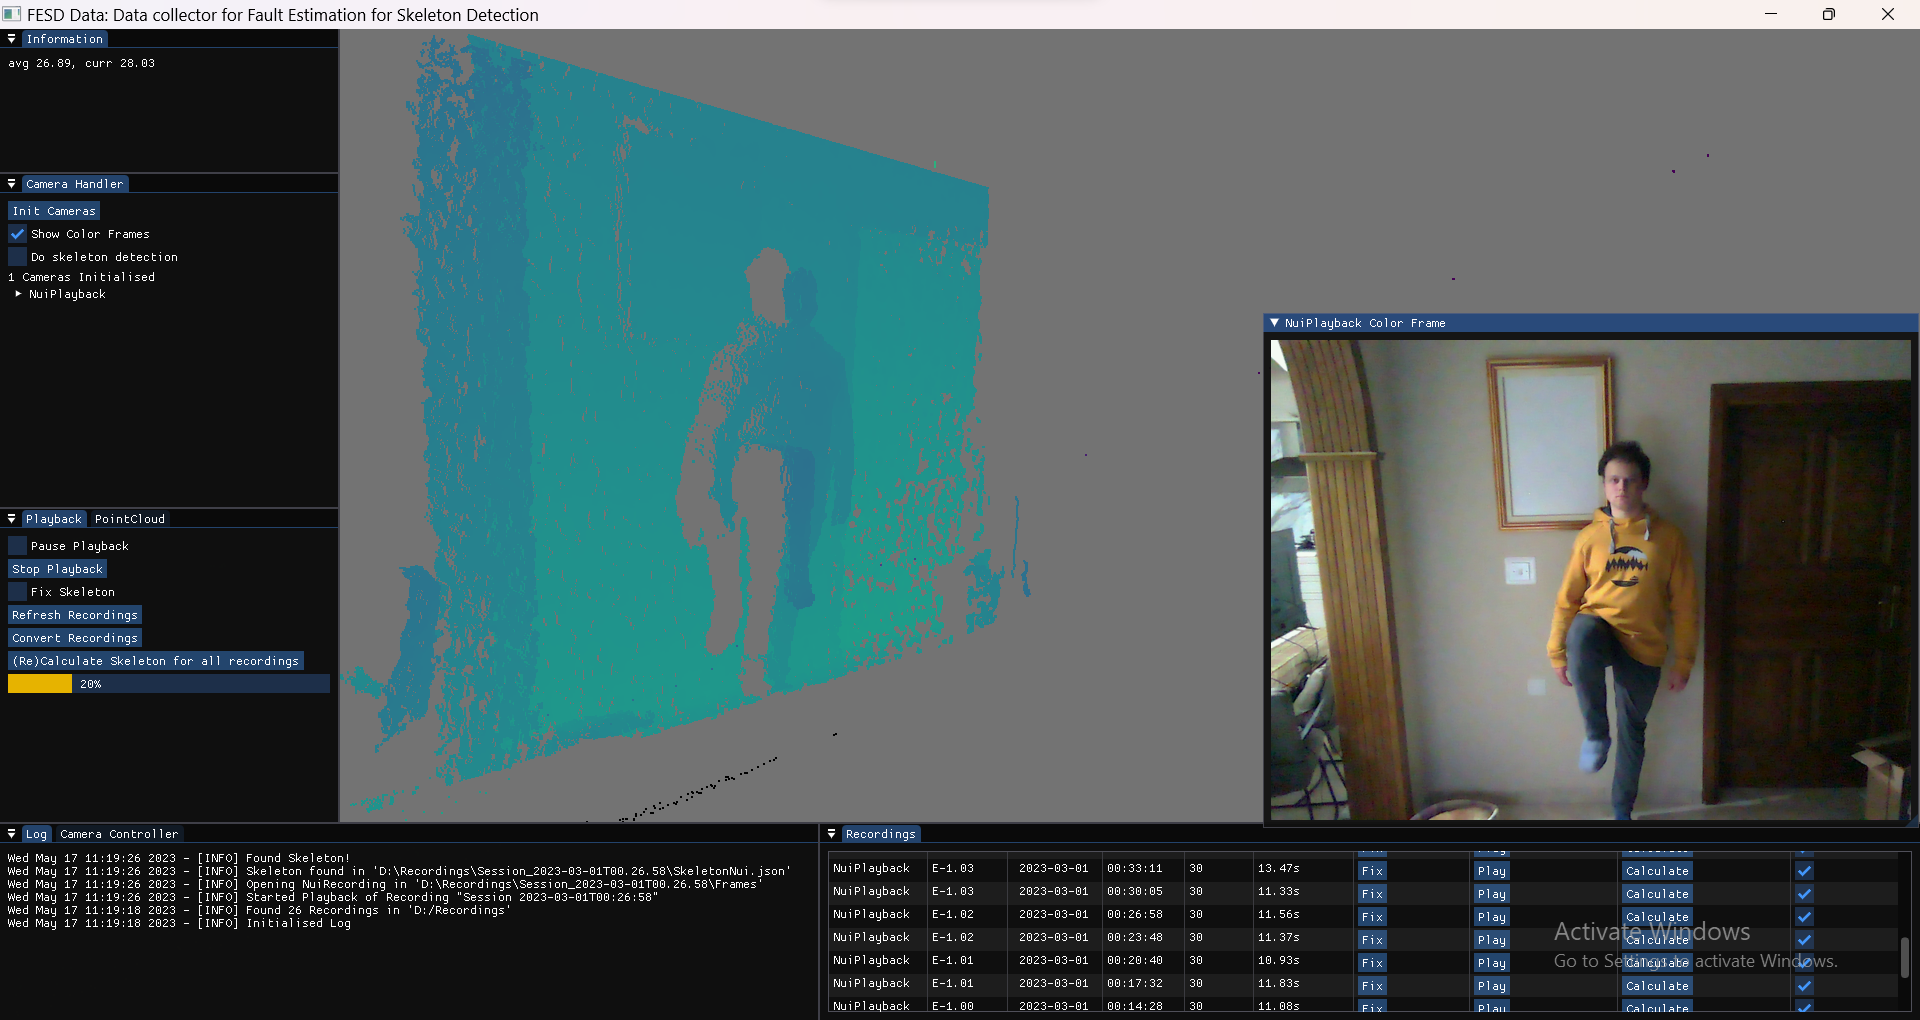
\includegraphics[width=.8\textwidth]{figures/FESDData/streaming.png}
  \caption[FESDData user interface for data streaming and recording]{The user interface of FESDData can be seen when streaming either a recording or a live feed of a camera. Both the RGB image, as well as the projected point cloud can be seen. At the bottom of the image, the list of recordings can be seen with a flag that indicates if the data has been labelled.}
  \label{fig:fesddata_recording}
\end{figure}

\begin{figure}
  \centering
  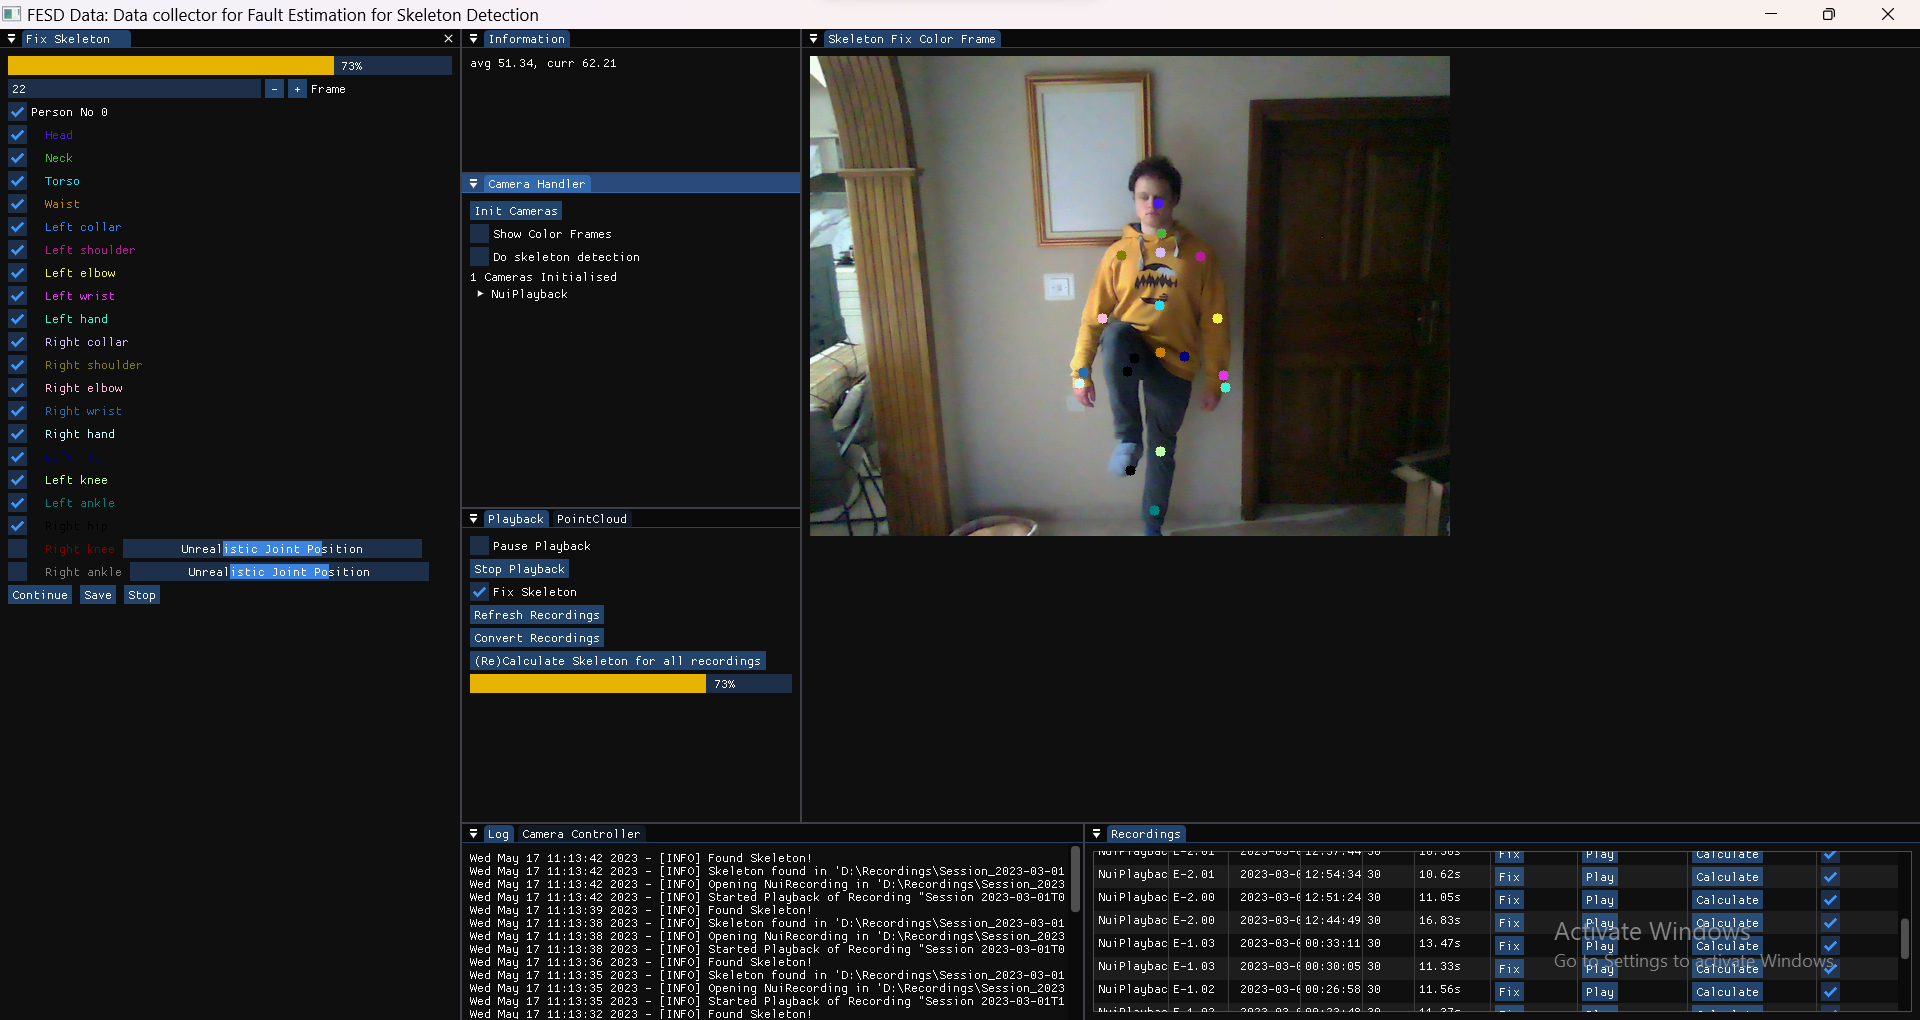
\includegraphics[width=.8\textwidth]{figures/FESDData/labelling.png}
  \caption[FESDData user interface for data labelling]{The user interface of FESDData during the labelling process. On the left, the actual labelling can be observed, where each joint, coloured according to the colour in the image, can be marked as erroneous or not. In this case, the left and right foot are in an incorrect position and are labelled as such. The right side contains a depiction of the joint positions as an overlay over the RGB image.}
  \label{fig:fesddata_labelling}
\end{figure}  
